\documentclass[a4paper, 10pt, ]{article}

\usepackage[slovak]{babel}

\usepackage[utf8]{inputenc}
\usepackage[T1]{fontenc}

\usepackage[left=4cm,
			right=4cm,
			top=2.1cm,
			bottom=2.6cm,
			footskip=7.5mm,
			twoside,
			marginparwidth=3.5cm,
			%showframe,
			]{geometry}

\usepackage{graphicx}
\usepackage[dvipsnames]{xcolor}

% ------------------------------

\usepackage{lmodern}

\usepackage[tt={oldstyle=false,proportional=true,monowidth}]{cfr-lm}

% ------------------------------

\usepackage{amsmath}
\usepackage{amssymb}
\usepackage{amsthm}

\usepackage{booktabs}
\usepackage{multirow}
\usepackage{array}
\usepackage{dcolumn}

\usepackage{natbib}

\usepackage[singlelinecheck=true]{subfig}


% ------------------------------


\usepackage{sectsty}
\allsectionsfont{\sffamily}


\usepackage{titlesec}
\titleformat{\paragraph}[hang]{\sffamily  \bfseries}{}{0pt}{}
\titlespacing*{\paragraph}{0mm}{3mm}{1mm}


\usepackage{fancyhdr}
\fancypagestyle{plain}{%
\fancyhf{} % clear all header and footer fields
\fancyfoot[C]{\sffamily {\bfseries \thepage}\ | {\scriptsize\oznacenieCasti}}
\renewcommand{\headrulewidth}{0pt}
\renewcommand{\footrulewidth}{0pt}}
\pagestyle{plain}


% ------------------------------


\makeatletter

	\def\@seccntformat#1{\protect\makebox[0pt][r]{\csname the#1\endcsname\hspace{5mm}}}

	\def\cleardoublepage{\clearpage\if@twoside \ifodd\c@page\else
	\hbox{}
	\vspace*{\fill}
	\begin{center}
	\phantom{}
	\end{center}
	\vspace{\fill}
	\thispagestyle{empty}
	\newpage
	\if@twocolumn\hbox{}\newpage\fi\fi\fi}

	\newcommand\figcaption{\def\@captype{figure}\caption}
	\newcommand\tabcaption{\def\@captype{table}\caption}

\makeatother


% ------------------------------


\def\naT{\mathsf{T}}

\hyphenpenalty=6000
\tolerance=6000


% ------------------------------


\usepackage[pdfauthor={},
			pdftitle={},
			pdfsubject={},
			pdfkeywords={},
			% hidelinks,
			colorlinks=true,
			breaklinks,
			]{hyperref}






% ------------------------------

\usepackage{enumitem}





\usepackage[titles]{tocloft}

\setlength{\cftsecindent}{-12mm}
\setlength{\cftsecnumwidth}{12mm}
\renewcommand{\cftsecpresnum}{\hfill}
\renewcommand{\cftsecaftersnum}{\hspace{4mm}}

\setlength{\cftsubsecindent}{-12mm}
\setlength{\cftsubsecnumwidth}{16mm} % 12 + 4
\renewcommand{\cftsubsecpresnum}{\hfill}
\renewcommand{\cftsubsecaftersnum}{\hspace{8mm}} % 4 + 4 mm

\setlength{\cftsubsubsecindent}{-12mm}
\setlength{\cftsubsubsecnumwidth}{20mm} % 12 + 4 + 4
\renewcommand{\cftsubsubsecpresnum}{\hfill}
\renewcommand{\cftsubsubsecaftersnum}{\hspace{12mm}} % 4 + 4 + 4 mm

\renewcommand{\cftsecpagefont}{\lstyle \bfseries}
\renewcommand{\cftsubsecpagefont}{\lstyle}
\renewcommand{\cftsubsubsecpagefont}{\lstyle}



\setlength{\cftparaindent}{-16mm}
\setlength{\cftparanumwidth}{28mm} % 16 + 4 + 4 + 4
\renewcommand{\cftparapresnum}{\hfill}
\renewcommand{\cftparaaftersnum}{\hspace{16mm}} % 4 + 4 + 4 + 4 mm

% ------------------------------









\usepackage{listings}



\renewcommand{\lstlistingname}{Výpis kódu}
\renewcommand{\lstlistlistingname}{Výpisy kódu}




%New colors defined below
\definecolor{codegreen}{rgb}{0,0.6,0}
\definecolor{codegray}{rgb}{0.5,0.5,0.5}
\definecolor{codepurple}{rgb}{0.58,0,0.82}
\definecolor{backcolour}{rgb}{0.95,0.95,0.95}

%Code listing style named "mystyle"
\lstdefinestyle{mystyle}{
  backgroundcolor=\color{backcolour},
  commentstyle=\fontfamily{lmtt}\fontsize{8.5pt}{8.75pt}\selectfont\color{codegreen},
  keywordstyle=\fontfamily{lmtt}\fontsize{8.5pt}{8.75pt}\selectfont\bfseries\color{Blue},
  stringstyle=\fontfamily{lmtt}\fontsize{8.5pt}{8.75pt}\selectfont\color{codepurple},
  basicstyle=\fontfamily{lmtt}\fontsize{8.5pt}{8.75pt}\selectfont,
  breakatwhitespace=false,
  breaklines=true,
  captionpos=t,
  keepspaces=true,
  numbers=left,
  numbersep=4mm,
  numberstyle=\fontfamily{lmtt}\fontsize{8.5pt}{8.75pt}\selectfont\color{lightgray},
  showspaces=false,
  showstringspaces=false,
  showtabs=false,
  tabsize=2,
  % xleftmargin=10pt,
  framesep=10pt,
  language=Python,
  escapechar=|,
}




% ------------------------------



\graphicspath{{fig/}{../../extObr/}}


\def\oznacenieCasti{cvUdK05 - ZS2019}





\begin{document}

\lstset{style=mystyle}





\fontsize{12pt}{22pt}\selectfont

\centerline{\textsf{Úvod do kybernetiky} \hfill \textsf{\oznacenieCasti}}

\fontsize{18pt}{22pt}\selectfont





\begin{flushleft}
    \textbf{\textsf{Prevodová charakteristika}}
\end{flushleft}



\normalsize

\bigskip

\tableofcontents

\bigskip

\vspace{18pt}












\begin{table}[b]
	\centering
	\catcode`\-=12

\caption{Hodnoty vstupného signálu}
\label{Hodnoty vstupného signálu}
\begin{tabular}{     c      c       }

\toprule
čas [s] & hodnota [kg m$^2$ s$^{-2}$] \\
\midrule
$0$ & $0,0$ \\
$10$ & $1,0$ \\
$30$ & $2,0$ \\
$20$ & $3,0$ \\
$40$ & $4,0$ \\
$50$ & $5,0$ \\
$60$ & $6,0$ \\
$70$ & $7,0$ \\
$80$ & $8,0$ \\
$95$ & $9,0$ \\
$110$ & $9,5$ \\
$135$ & $9,81$ \\
\bottomrule
\end{tabular}
\end{table}







\section{O meraní prevodovej charakteristiky}


\noindent
Prevodová charakteristika je závislosť ustálených hodnôt výstupnej veličiny od ustálených hodnôt vstupnej veličiny. Zhruba povedané. Prevodová charakteristika, niekde sa nazýva aj statická charakteristika, teda charakterizuje systém len v~ustálených stavoch. Neobsahuje informáciu o dynamike systému.


V nasledujúcom sa pokúsime načrtnúť meranie prevodovej charakteristiky - tu sa však nebude naozaj niečo merať, ale reálny systém bude nahradený simulovaným. Proces získavania „surových“ dát, ktoré sú potrebné pre určenie prevodovej charakteristiky a proces spracovania týchto dát bude však rovnaký akoby išlo o reálny systém.

Systém, ktorý bude predmetom skúmania, ktorého prevodovú charakteristiku budeme merať, je kyvadlo, tak ako bolo už skôr opísané. Navyše však bude k výstupnej veličine simulováného systému pridaný čitateľovi neznámy šum. Dôvodom je lepšie napodobenie situácie v akej by bol čitateľ ak by sa zaoberal výstupnou veličinou reálneho systému.


















\subsection{Úlohy}

\begin{enumerate}

	\item Vytvorte numerickú simuláciu časového priebehu výchylky kyvadla. Je zrejmé, že nie je dôvod uvažovať nenulové začiatočné podmienky, a teda $\varphi = 0$ [rad] a~$\dot\varphi = 0$ [rad/s]. Vstupný signál $u(t) = 0$ [kg~m$^2$~s$^{-2}$] sa bude meniť podľa potreby.


    \item Odmerajte (simulačne) prevodovú charakteristiku uvažovaného systému.

\end{enumerate}












\begin{figure}[!t]
	\centering

    \makebox[\textwidth][c]{%
	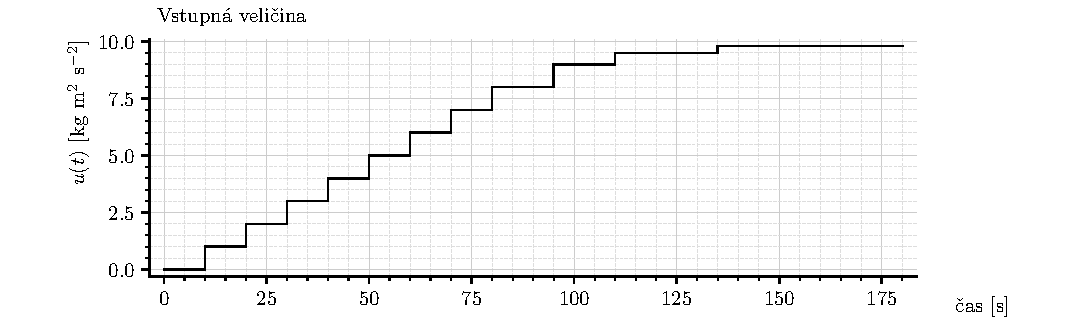
\includegraphics{../fig/cv04_fig_1.pdf}
	}

	\caption{Priebeh vstupného signálu}
	\label{Priebeh vstupného signálu}

\end{figure}















\begin{figure}[!b]
	\centering


    \makebox[\textwidth][c]{%
	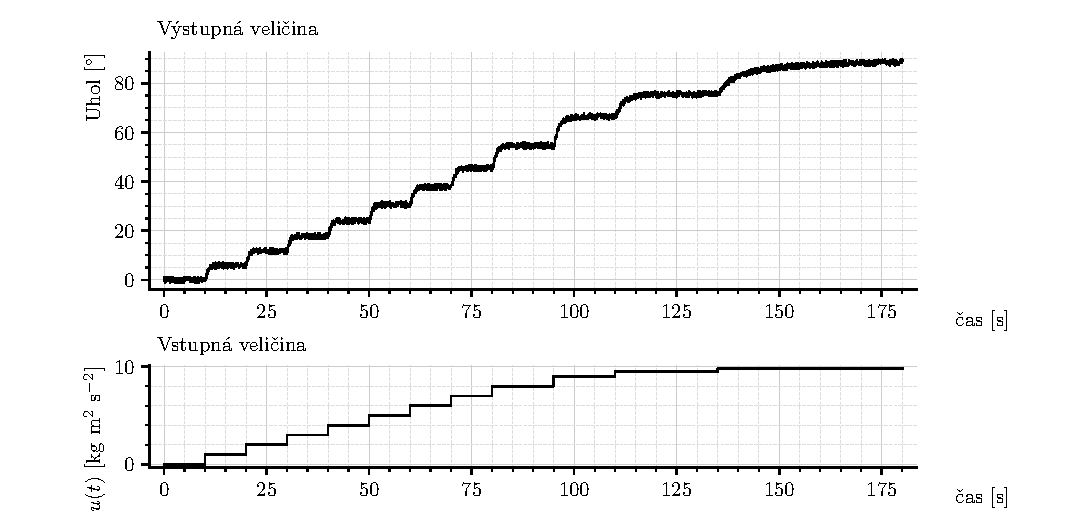
\includegraphics{../fig/cv04_fig_2.pdf}
	}

	\caption{Surové dáta}
	\label{Surové dáta}

\end{figure}






\subsection{Surové dáta...}

Ako už bolo uvedené, predmetom záujmu sú ustálené hodnoty výstupného signálu. Ak na vstup privedieme vstupný signál s nejakou konštantnou vstupnou hodnotou, následne počkáme istý čas nech sa výstupný signál ustáli, tak potom môžeme odčítať (odmerať) ustálenú hodnotu výstupného signálu. Takto sa získa jeden bod z prevodovej charakteristiky.








Hneď potom je však možné zmeniť hodnotu vstupného signálu a opäť čakať, kým sa výstup ustáli.

Tento postup, hodnoty vstupného signálu a doby, počas ktorých sa „čaká“ na ustálenie výstupu, možno vyjadriť tabuľkou nasledovne. Prvý stĺpec je čas, v ktorom sa zmení (prepne) vstup a druhý stĺpec je hodnota (konštanta), na ktorú sa zmení (prepne).


Z uvedeného je zároveň jasné, že interval vstupných hodnôt, pre ktorý zisťujeme ustálené hodnoty výstupu je $0$ až $9,81$ [kg m$^2$ s$^{-2}$]. Iné by vzhľadom na konkrétne kyvadlo, ktoré sa tu uvažuje, malo pramalý význam.

Vstupný signál tak ako je definovaný tabuľkou~\ref{Hodnoty vstupného signálu} možno znázorniť ako na obr.~\ref{Priebeh vstupného signálu}.





Simulujme teraz priebeh výstupnej veličiny kyvadla (výchylky kyvadla) pri uvedenom vstupnom signály. Výsledok je na obr.~\ref{Surové dáta}.
























\subsection[Spracovanie surových dát]{Spracovanie surových dát - odčítanie („z grafu“, z dát) bodov prevodovej charakteristiky}


Zo surových dát je potrebné získať jednotlivé body prevodovej charakteristiky. To v~prvom rade znamená byť schopný odčítať ustálenú hodnotu výstupného signálu (zo surových dát). Pre ilustráciu, venujme sa nameraným dátam od desiatej sekundy po dvadsiatu sekundu, teda pre interval, počas ktorého bola na vstupe hodnota $u=1$ [kg m$^2$ s$^{-2}$]. Táto časť dát je nakreslená na obr.~\ref{Surové dáta - detail}.

\begin{figure}[!ht]
	\centering



    \makebox[\textwidth][c]{%
	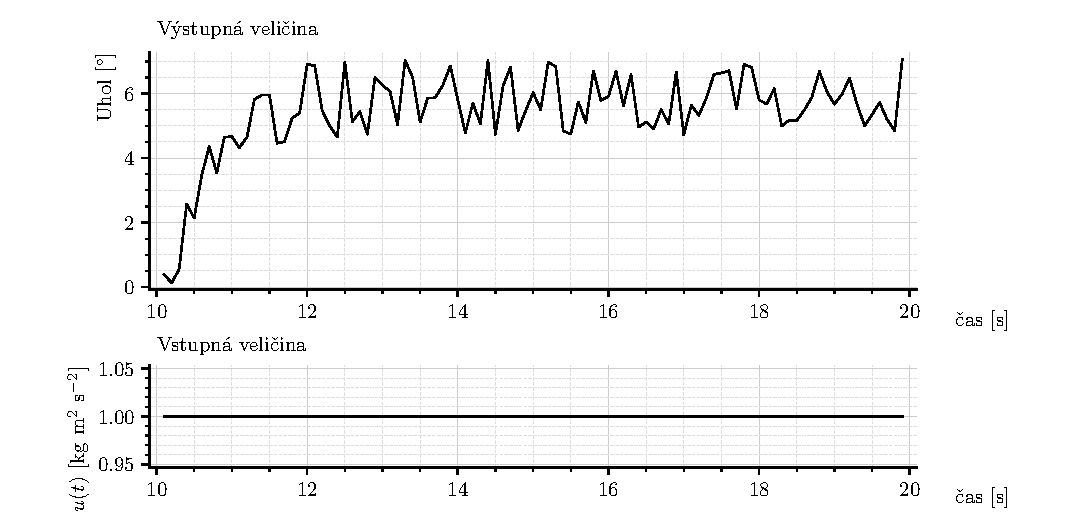
\includegraphics{../fig/cv04_fig_3.pdf}
	}



	\caption{Surové dáta - detail}
	\label{Surové dáta - detail}



\end{figure}


Z obr.~\ref{Surové dáta - detail} je zrejmé, že v poslednej tretine intervalu je už možné považovať hodnotu výstupu za ustálenú. Vyznačme túto časť dát - viď obr.~\ref{Surové dáta - detail2}.

\begin{figure}[!ht]
	\centering

    \makebox[\textwidth][c]{%
	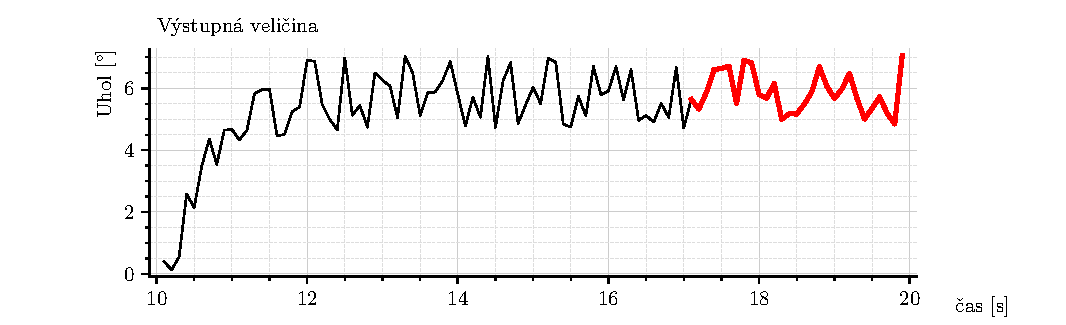
\includegraphics{../fig/cv04_fig_4.pdf}
	}

    \vspace{-6pt}

	\caption{Surové dáta - detail}
	\label{Surové dáta - detail2}

\end{figure}


Otázka je, ako z vyznačeného úseku určiť jednu hodnotu - ustálenú hodnotu. Prirodzenou voľbou je urobiť priemer z vybranej (vyznačenej) časti dát. Priemer je vyznačený na obr.~\ref{Surové dáta - detail3}



\begin{figure}[!ht]
	\centering

    \makebox[\textwidth][c]{%
	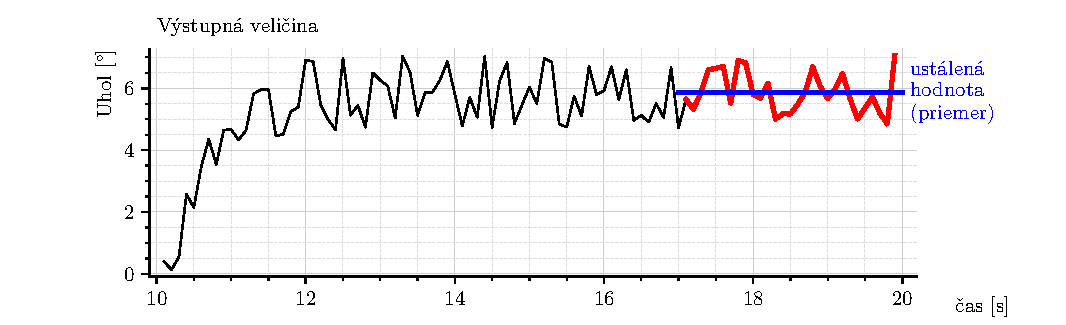
\includegraphics{../fig/cv04_fig_5.pdf}
	}

    \vspace{-6pt}

	\caption{Surové dáta - detail}
	\label{Surové dáta - detail3}

    \vspace{-6pt}

\end{figure}




Rovnako je samozrejme možné postupovať pri všetkých bodoch prevodovej charakteristiky. Všetky ustálené hodnoty odčítané zo „surových dát“ sú znázornené na obr.~ \ref{Surové dáta2}.


\begin{figure}[!ht]
	\centering

    \vspace{-6pt}

    \makebox[\textwidth][c]{%
	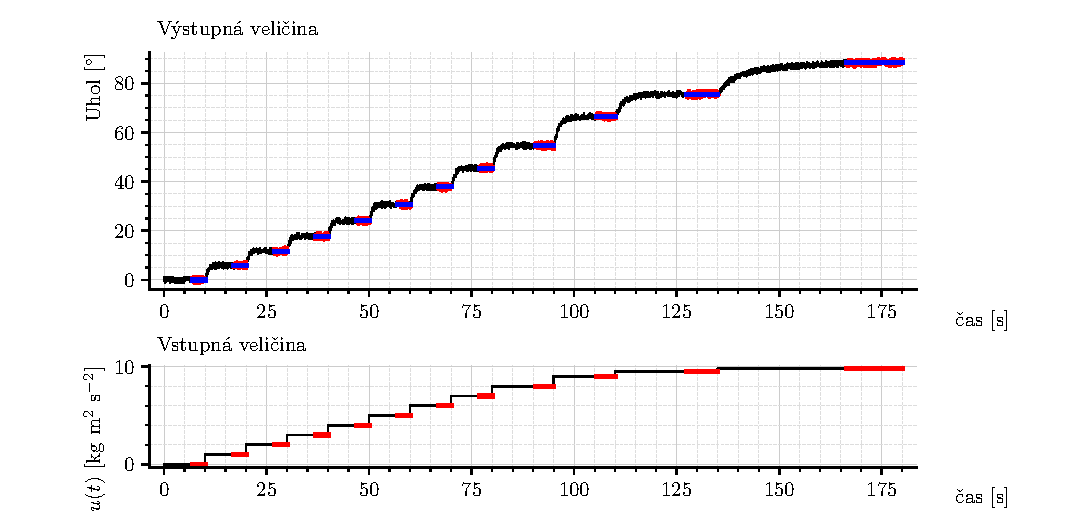
\includegraphics{../fig/cv04_fig_6.pdf}
	}

    \vspace{-6pt}

	\caption{Surové dáta}
	\label{Surové dáta2}

    \vspace{-6pt}

\end{figure}



Odčítané hodnoty sú následne uvedené v tabuľke~\ref{Prevodová charakteristika}. Prevodová charakteristika je graficky znázornená na obr.~\ref{Prevodová charakteristika graf}.





\begin{table}[!ht]
	\centering
	\catcode`\-=12

\caption{Prevodová charakteristika}
\label{Prevodová charakteristika}


\vspace{-2mm}


\begin{tabular}{     c      c       }
\toprule
vstup [kg m$^2$ s$^{-2}$] & výstup [°] \\
\midrule
$0,0$ & $0,00691$\\
$1,0$ & $5,7$\\
$2,0$ & $11,8$\\
$3,0$ & $17,7$\\
$4,0$ & $24,3$\\
$5,0$ & $30,6$\\
$6,0$ & $37,6$\\
$7,0$ & $45,2$\\
$8,0$ & $54,5$\\
$9,0$ & $66,5$\\
$9,5$ & $75,6$\\
$9,81$ & $88,7$\\
\bottomrule
\end{tabular}
\end{table}



\begin{figure}[!ht]
	\centering

    \makebox[\textwidth][c]{%
	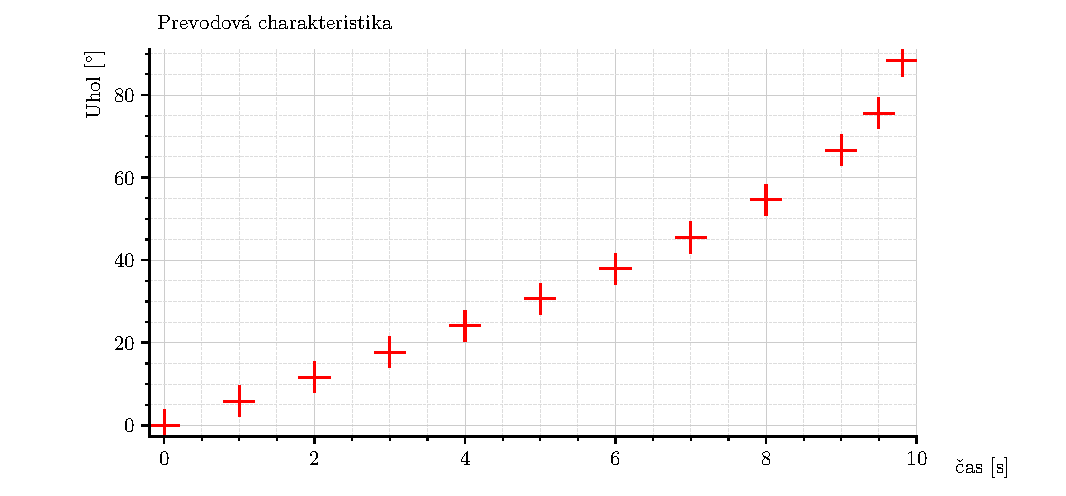
\includegraphics{../fig/cv04_fig_7.pdf}
	}

    \vspace{-6mm}

	\caption{Prevodová charakteristika}
	\label{Prevodová charakteristika graf}

\end{figure}








\clearpage



\section{Doplnkový text: o aproximácii prevodovej charakteristiky lineárnym modelom}




\noindent
Majme nameranú prevodovú charakteristiku, dáta sú v tabuľke~\ref{Prevodová charakteristika}. Prevodová charakteristika je graficky znázornená na obr.~\ref{Prevodová charakteristika graf}.







\subsection{Model}

Body prevodovej charakteristiky zodpovedajú istej vlastnosti reálneho systému (reálne existujúceho systému). Zodpovedajú závislosti výstupu systému od vstupu systému, samozrejme v ustálenom stave. Nameraných je však len niekoľko bodov. V týchto bodoch je daná vlastnosť systému známa. Čo však v prípade ak by bolo potrebné poznať danú vlastnosť mimo nameraných bodov? Teda mimo hodnôt vstupu, pre ktoré bola prevodová charakteristika nameraná.

Aj pre tieto účely je výhodné využiť model. Model reálnej vlastnosti systému. Samotnej vlastnosti systému zodpovedá nameraná závislosť (prevodová charakteristika). Aproximáciou tejto závislosti je možné získať model.

Model nech je v tomto prípade matematický vzťah, funkčná závislosť, istý predpis... Ak hodnota na vstupe modelu bude rovnaká ako hodnota na vstupe reálneho systému, potom hodnota na výstupe modelu nech je „približne rovnaká“ ako hodnota reálna. Toto nech však platí pre všetky namerané body prevodovej charakteristiky. Teda model nech sa približne zhoduje s reálnymi dátami. Ak toto platí v nameraných bodoch, potom to, zrejme, platí aj v iných bodoch. Platí to pre akúkoľvek hodnotu na vstupe modelu - že výstup modelu sa približne zhoduje s reálnym výstupom systému.



Takto všeobecne opísaný model možno skonkretizovať napríklad nasledovne: Nech modelom je polynomiálna funkcia
\begin{equation} \label{polyFcnDef}
    \hat y = \Theta_3 u^3 + \Theta_2 u^2 + \Theta_1 u + \Theta_0
\end{equation}
kde „vstup modelu“ je $u$ a „výstup modelu“ je $\hat y$. Parametrami modelu sú koeficienty (čísla) $\Theta_3$, $\Theta_2$, $\Theta_1$ a $\Theta_0$.

Mimochodom, ide o lineárny model. Parametre modelu sú v lineárnom vzťahu k~„signálom“ modelu (k~vstupom modelu).






\subsection{Jednoduché hľadanie parametrov (koeficientov) polynómu}

V tejto časti sa použije MATLAB pre nájdenie parametrov (koeficientov) polynomiálnej funkcie \eqref{polyFcnDef}. Pre tieto účely majme premennú \verb|prevodChar|, ktorej prvý stĺpec sú hodnoty vstupnej veličiny a druhý stĺpec sú hodnoty výstupnej veličiny. Teda obr.~\ref{Prevodová charakteristika graf} by sme v MATLABe nakreslili takto
\begin{lstlisting}[language=Matlab,]
figure(1);
plot(prevodChar(:,1), prevodChar(:,2), '+r');
\end{lstlisting}






\subsubsection{Funkcia polyfit}

Funkcia \verb|polyfit| slúži vo všeobecnosti na hľadanie koeficientov polynómu (polynomiálnej funkcie) daného stupňa tak aby polynomiálna funkcia aproximovala dané dáta (napr. nameranú x-y závislosť). Kritériom pre hľadanie koeficientov je minimalizácia štvorcov (kvadrátov) odchýlok medzi nameranou hodnotou a jej aproximáciou. Presnejšie, minimalizácia sumy štvorcov odchýlok.

Použitie funkcie \verb|polyfit| v tu uvažovanom konkrétnom prípade by bolo nasledovné
\begin{lstlisting}[language=Matlab,]
polyKoef = polyfit(prevodChar(:,1),prevodChar(:,2), 3)
\end{lstlisting}
a premenná \verb|polyKoef| obsahuje hodnoty koeficientov polynómu. Rovnica \eqref{polyFcnDef} s~nájdenými koeficientami je:
\begin{equation} \label{modelPolifitVysl}
    \hat y = 0,1111 u^3  -1,1150 u^2 + 8,9102 u  -1,1770
\end{equation}






\subsubsection{Funkcia polyval}

Pre vypočítanie hodnôt (výstupov) $\hat y$ pre požadované vstupy $u$ je možné použiť funkciu \verb|polyval|. Ak teda chceme ku každému vstupu, pre ktorý bola nameraná hodnota výstupu, vypočítať jej aproximáciu $\hat y$ podľa modelu \eqref{modelPolifitVysl}, potom stačí zavolať:
\begin{lstlisting}[language=Matlab,]
y_hat = polyval(polyKoef, prevodChar(:,1));
\end{lstlisting}
Obrázok, na ktorom sú naraz zobrazené namerané dáta aj výstup modelu \eqref{modelPolifitVysl} možno nakresliť nasledovne:
\begin{lstlisting}[language=Matlab,]
figure(2);
hold on;
plot(prevodChar(:,1), prevodChar(:,2), '+r')
plot(prevodChar(:,1), y_hat, '.b')
\end{lstlisting}
Samotný obrázok by bol podobný obr.~\ref{Prevodová charakteristika namer vs model}





\begin{figure}[!ht]
	\centering

    \makebox[\textwidth][c]{%
	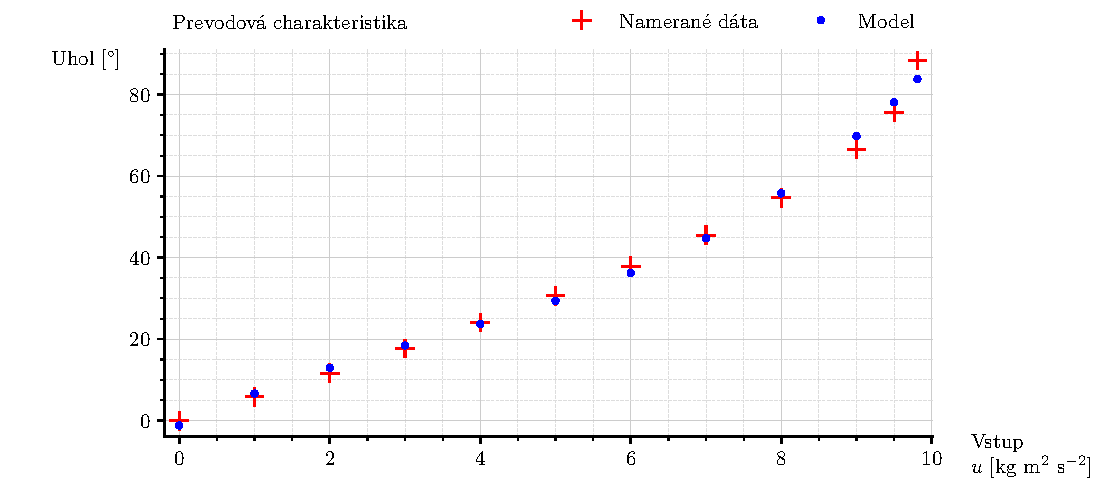
\includegraphics{../fig/cv06_fig_2.pdf}
	}

    \vspace{-4mm}

	\caption{Prevodová charakteristika}
	\label{Prevodová charakteristika namer vs model}

\end{figure}





\subsubsection{Používanie modelu}

Model, samozrejme, umožňuje vypočítať aproximáciu reálneho výstupu pre akúkoľvek hodnotu vstupu - nie len pre hodnoty vstupov, pre ktoré boli merané hodnoty skutočného systému. Vypočítajme výstupy modelu pre tieto vstupné hodnoty (dané vektorom):
\begin{lstlisting}[language=Matlab,]
u_ine = [0:0.1:9.81];
\end{lstlisting}
Teda zavoláme funkciu \verb|polyval|.
\begin{lstlisting}[language=Matlab,]
y_ine_1 = polyval(polyKoef, u_ine);
\end{lstlisting}
Nakreslime obrázok (viď obr.~\ref{Prevodová charakteristika nuine})
\begin{lstlisting}[language=Matlab,]
figure(3);
hold on;
plot(prevodChar(:,1), prevodChar(:,2), '+r')
plot(u_ine, y_ine_1, '.b')
\end{lstlisting}




\begin{figure}[!ht]
	\centering

    \makebox[\textwidth][c]{%
	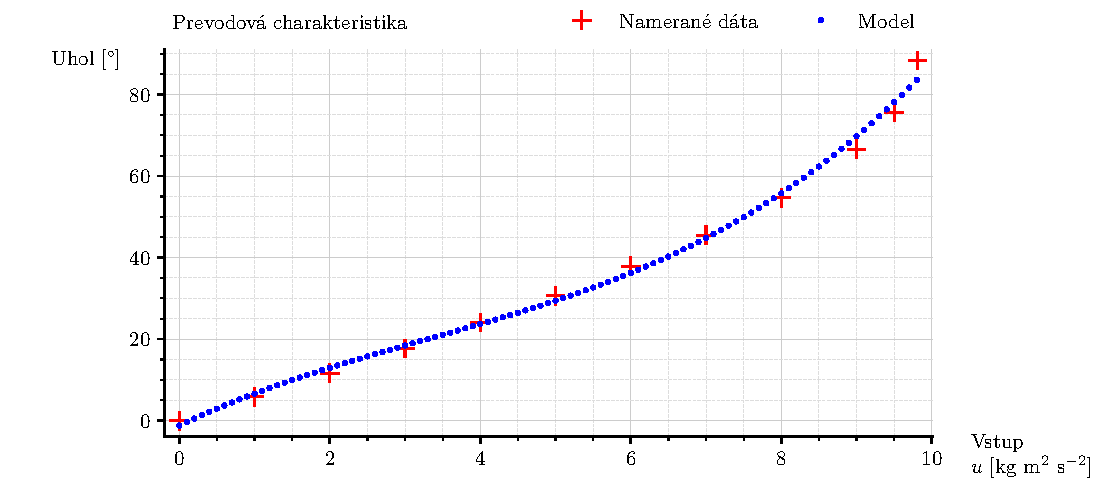
\includegraphics{../fig/cv06_fig_3.pdf}
	}

    \vspace{-4mm}

	\caption{Prevodová charakteristika}
	\label{Prevodová charakteristika nuine}

\end{figure}









\subsection{Čo vlastne robí funkcia polyfit}

V MATLABe funkcia \verb|polyfit| zostaví istú sústavu rovníc a následne sa použije, pre MATLAB ikonický, príkaz „backslash“: \verb|\|. Dokonca niektorí ľudia nosia na tričku nápis (niektorí nie, pretože také tričko nemajú): \verb|x = A\b;|


O tom, že funkcia \verb|polyfit| používa príkaz „backslash“, sa čitateľ môže ľahko presvedčiť otvorením súboru, v ktorom je funkcia definovaná. Stačí zadať príkaz (do Command Window):
\begin{lstlisting}[language=Matlab,]
open polyfit
\end{lstlisting}
Otvorí sa súbor \verb|polyfit.m| a na riadku číslo 65 sa používa príkaz „backslash“.






\subsubsection{Preurčená sústava rovníc}

Tu sa pokúsime naznačiť, akú sústavu rovníc zostaví a~potom rieši funkcia \verb|polyfit| aby našla to čo hľadá - hľadá koeficienty polynómu v~zmysle istého kritéria (minimalizovať sumu štvorcov odchýlok medzi nameranými dátami a výstupom modelu).

Podobne sa dá postupovať nie len práve pri hľadaní nejakých koeficientov polynómu. Podobný postup je možné použiť pri hľadaní parametrov lineárneho modelu vo všeobecnosti. Pritom však dôkladnejšie vysvetlenie pojmu \emph{lineárny model} a~\emph{identifikácia} jeho parametrov je praďaleko nad rámec tohto textu, predmetu, a~asi aj bakalárskeho študijného programu.

Akokoľvek, aspoň náznak pre ilustráciu istotne má zmysel.


Preurčená sústava rovníc je sústava algebraických rovníc, taká, že počet rovníc je väčší ako počet neznámych. Tu by bolo možné pridať značné množstvo detailov. Na niektoré si azda čitateľ spomína zo svojho štúdia lineárnej algebry.

Ak má sústava rovníc toľko neznámych koľko rovníc, potom je riešenie jednoznačné (iba ak by nebolo).

Ak má sústava rovníc menej neznámych ako je počet rovníc, potom riešenie pri prvom intuitívnom priblížení neexistuje. Avšak sú prípady, keď je potrebné „aspoň nejako“ vyriešiť takúto sústavu rovníc. Taký prípad sa vyskytuje napríklad aj pri používaní funkcie \verb|polyfit| tak ako bola použitá vyššie.

Preurčenú sústavu rovníc je možné riešiť v zmysle tzv. \emph{metódy najmenších štvorcov}. Algebraický pohľad na vec tu vynechajme, ale aplikovanie tejto „metódy“ sa v našom prípade prejaví tak, že suma štvorcov odchýlok medzi nemeranými dátami a výstupom modelu je minimálna možná.








\bigskip

Pripomeňme, že sa zaoberáme prípadom, keď modelom je polynomiálna funkcia v~tvare
\begin{equation}
    \hat y = \Theta_3 u^3 + \Theta_2 u^2 + \Theta_1 u + \Theta_0
\end{equation}
čo je rovnica \eqref{polyFcnDef} a teda „vstup modelu“ je $u$ a „výstup modelu“ je $\hat y$. Parametrami modelu sú koeficienty (čísla) $\Theta_3$, $\Theta_2$, $\Theta_1$ a $\Theta_0$.


Ak by sme na vstup modelu priviedli hodnotu zodpovedajúcu prvému bodu prevodovej charakteristiky (súradnice bodu označme $[u_1, y_1]$) potom na výstupe modelu by bola hodnota, ktorú označme $\hat y_1$. Presnejšie napísané:
\begin{equation}
    \hat y_1 = \Theta_3 u_1^3 + \Theta_2 u_1^2 + \Theta_1 u_1 + \Theta_0
\end{equation}
Pre druhý bod prevodovej charakteristiky by to bolo
\begin{equation}
    \hat y_2 = \Theta_3 u_2^3 + \Theta_2 u_2^2 + \Theta_1 u_2 + \Theta_0
\end{equation}
atď\ldots

Samozrejme, model má v každom prípade len jednu sadu parametrov: $\Theta_3$, $\Theta_2$, $\Theta_1$ a $\Theta_0$. Tie, samozrejme, ostávajú rovnaké bez ohľadu na to aký je vstup modelu.




Model má aproximovať reálne dáta (reálnu vlastnosť systému). Odchýlky medzi modelom a dátami v jednotlivých nameraných bodoch sú:
\begin{subequations}
    \begin{align}
        e_1 &= y_1 - \hat y_1 \\
        e_2 &= y_2 - \hat y_2 \\
        e_3 &= y_3 - \hat y_3 \\
        &\vdots
    \end{align}
\end{subequations}
Odchýlky teda sú $e_1$, $e_2$, atď. Za $\hat y_i$, pre $i = 1,\ldots, N$, možno dosadiť vyššie uvedené, teda
\begin{subequations}
    \begin{align}
        e_1 &= y_1 - \Theta_3 u_1^3 + \Theta_2 u_1^2 + \Theta_1 u_1 + \Theta_0 \\
        e_2 &= y_2 - \Theta_3 u_2^3 + \Theta_2 u_2^2 + \Theta_1 u_2 + \Theta_0 \\
        e_3 &= y_3 - \Theta_3 u_3^3 + \Theta_2 u_3^2 + \Theta_1 u_3 + \Theta_0 \\
        &\vdots \\
        e_N &= y_N - \Theta_3 u_N^3 + \Theta_2 u_N^2 + \Theta_1 u_N + \Theta_0
    \end{align}
\end{subequations}

Ak by sa model presne zhodoval s dátami, potom by platilo
\begin{subequations}
    \begin{align}
        e_1 &= 0 \\
        &\vdots \\
        e_N &= 0
    \end{align}
\end{subequations}
Toto by však bol úplne ideálny prípad a dá sa tušiť, že takýto prípad nenastane.

Akokoľvek, čo sa týka číselných hodnôt $e_i$ považujme ich na chvíľku za známe, také, že sú nulové. Potom práve vznikla sústava rovníc. Ich počet je $N$. Neznáme v rovniciach sú $\Theta_3$, $\Theta_2$, $\Theta_1$ a $\Theta_0$, teda 4 neznáme. Všetko ostatné je v rovniciach známe, teda známe sú $e_i$, $y_i$ aj $u_i$. V tomto prípade, počet rovníc je väčší ako počet neznámych. To je veľmi dôležité, avšak prečo je to dôležité je ďalšia vec čo začína byť nad rámec tohto textu.

Uvedená sústava rovníc sa dá zapísať maticovo:
\begin{equation} \label{detailPreurcVseob}
    \begin{bmatrix}
        0 \\ 0 \\\vdots \\ 0
    \end{bmatrix}
    =
    \begin{bmatrix}
        y_1 \\ y_2 \\\vdots \\ y_N
    \end{bmatrix}
    -
    \begin{bmatrix}
        u_1^3 & u_1^2 & u_1 & 1 \\
        u_2^3 & u_2^2 & u_2 & 1 \\
        \vdots & \vdots & \vdots & \vdots \\
        u_N^3 & u_N^2 & u_N & 1
    \end{bmatrix}
    \begin{bmatrix}
        \Theta_3 \\ \Theta_2 \\ \Theta_1 \\ \Theta_0
    \end{bmatrix}
\end{equation}
Pre zjednodušenie zaveďme označenia:
\begin{equation}
    0 = y - H \Theta
\end{equation}
kde je snáď zrejmé čo je čo. Inak zapísané:
\begin{equation} \label{psrtem}
    H \Theta = y
\end{equation}

Toto je (pri predpoklade o vyššom počte rovníc ako je neznámych) sústava rovníc, ktorú je možné riešiť v zmysle metódy najmenších štvorcov (kvadrátov). Podrobnosti sú ďaleko praďaleko nad rámec tohto textu. Výsledkom však je, že vektor $y$ a vektor $H \Theta$ (áno je to vektor) sa „rovnajú“ v takom zmysle, že suma kvadrátov odchýlok medzi ich súradnicami je minimálna možná. Inak, a užitočnejšie, povedané, $y - H \Theta$ je vlastne $e$. Vektor $e$ obsahuje všetky odchýlky medzi modelom a nameranými dátami. Vektor $e$ sú ale aj odchýlky medzi súradnicami vektorov, o ktorých sme práve hovorili. A suma kvadrátov týchto odchýlok je minimálna! Takže aj suma odchýlok medzi modelom a dátami je minimálna!






\subsubsection{Názorná ukážka}

Zostavme teraz, v MATLABe, maticu $H$ a vektor $y$ podľa toho čo ukazuje rovnica \eqref{detailPreurcVseob}.
\begin{lstlisting}[language=Matlab,]
H = [prevodChar(:,1).^3, prevodChar(:,1).^2, prevodChar(:,1).^1, ones(length(prevodChar(:,1)), 1)];
y = prevodChar(:,2);
\end{lstlisting}
Neznámu nazvime \verb|Theta| a riešenie preurčeného systému rovníc \eqref{psrtem} hľadajme príkazom:
\begin{lstlisting}[language=Matlab,]
Theta = H\y
\end{lstlisting}
Výsledkom je:
\begin{lstlisting}[language=Matlab,]
Theta =

    0.1111
   -1.1150
    8.9102
   -1.1770
\end{lstlisting}
a to sú také isté hodnoty koeficientov ako sa uvádza v rovnici \eqref{modelPolifitVysl}.







\subsubsection{Analytické riešenie}

V predchádzajúcej časti sme použili istý príkaz („backslash“) pre hľadanie riešenia preurčeného systému algebraických rovníc v zmysle metódy najmenších štvorcov. Čo presne robí tento príkaz, aby našiel riešenie, je opäť raz ďaleko nad rámec tohto textu. Ak by sme však hľadali riešenie formulovaného problému analyticky, je možné ukázať (ale nebudeme to robiť), že to vedie na nasledujúcu rovnicu
\begin{equation}
    \Theta = \left( H^\mathsf T H \right)^{-1} H^\mathsf T y
\end{equation}
Táto rovnica je známa pod názvom \emph{Gaussov vzorec}.

Pri použití tejto rovnice je potrebné urobiť inverziu istej matice - ako je zrejmé\ldots \  Práve táto inverzia matice môže byť (a v praxi veľmi často je) z~hľadiska numerických výpočtov veľmi náročnou operáciou (a napríklad aj toto rieši efektívnejšie príkaz „backslash“).

Použime tento vzorec (rovnicu) priamo v MATLABe:
\begin{lstlisting}[language=Matlab,]
Theta_1 = inv(H'*H)*H'*y
\end{lstlisting}
Výsledkom je:
\begin{lstlisting}[language=Matlab,]
Theta_1 =

    0.1111
   -1.1150
    8.9102
   -1.1770
\end{lstlisting}
a to sú opäť také isté hodnoty koeficientov ako sa uvádza v rovnici \eqref{modelPolifitVysl}.








\subsection{Všetko uvedené realizované v jazyku Python}


Nasledujúce je ukážkou príkazov v jazyku Python, kde sa využíva knižnica (modul) \verb|numpy|. Príkazy realizujú to isté ako bolo uvedené doposiaľ (pomocou príkazov v~MATLABe). Kreslenie obrázkov je tu vynechané\ldots



\begin{lstlisting}[language=Python,]
import numpy as np


# pouzitie funkcie polyfit (z modulu numpy)
polyKoef = np.polyfit(prevodChar[:,0],prevodChar[:,1], 3)


# funkcia polyval pouzita pre vypocet aproximacie nameranych hodnot vystupu
y_hat = np.polyval(polyKoef, prevodChar[:,0])


# vypocitanie aproximacie vystupu pre rozne vstupne hodnoty
u_ine = np.arange(0,9.81,0.1)
y_ine_1 = np.polyval(polyKoef, u_ine)


# zostavenie matice H a vektora y

H = np.hstack([
        (prevodChar[:,0].reshape(-1,1))**3,
        (prevodChar[:,0].reshape(-1,1))**2,
        prevodChar[:,0].reshape(-1,1),
        np.ones([prevodChar[:,0].shape[0],1]),
        ])

y = prevodChar[:,1].reshape(-1,1)


# Riesenie preurceneho systemu rovnic v zmysle metody najmensich stvorcov
Theta = np.linalg.lstsq(H, y, rcond=None)[0]

# Pouzitie Gaussovho vzorca
Theta_1 = np.matmul(np.matmul(np.linalg.inv(np.matmul(H.T, H)), H.T), y)

\end{lstlisting}












\end{document}
